\chapter{Architettura dei processori}
I processori che sono utilizzati al giorno d'oggi sono vari e possono essere contraddistinti in base al loro sistema di funzionamento, in base alla tipologia di codici operativi che possono essere utilizzati (ISA - Instruction Set Architecture) e dalla tipologia di architettura adottata (CISC o RISC). 
In generale, però, l'architettura di un processore, internamente, non cambia, ciò che può cambiare sono le modalità con cui tale processore va ad eseguire le istruzioni in un certo modo. Tale capitolo, quindi, non avrà solo lo scopo di introdurre le architetture dei processori più utilizzate, ma avrà anche lo scopo di definire quali tra le scelte disponibili, sono più efficienti o veloci ed il perchè di tali considerazioni.
\section{Generalità sul processore}
Il processore, di per se, è un componente atto ad eseguire dei codici operativi predefiniti all'interno della sua ISA.
Oltre al codice operativo, in un processore, vi è anche la sua \textbf{architettura}, che può essere di vario tipo. In generale un processore, a livello architetturale, è formata dai seguenti componenti:
\begin{itemize}
    \item \textbf{Unità di controllo}: Determina i passi elementari che deve fare un processore al fine di eseguire un istruzione
    \item \textbf{Registro Program Counter}: Registro contenente il puntatore alla prossima istruzione
    \item \textbf{Registro Istruction Register}: Registro contenente l'istruzione che sta venendo eseguita
    \item \textbf{Registro Memory Address}: Registro di interfacciamento con la memoria, per gli indirizzi
    \item \textbf{Registro Memory Buffer}: Registro di interfacciamento della memoria, per i dati
    \item \textbf{Registri dato ad uso generico}: Registri dato e indirizzo presenti nell'architettura
    \item \textbf{Unità Logico-Aritmetica (ALU)}: Unità che permette le esecuzioni, dati gli operandi, di operazioni logico-aritmetiche
\end{itemize}

In particolare, per l'\textbf{Unità Logico Aritmetica}, vi è un'interazione anche con un altro registro all'interno della stessa architettura, ovvero il registro di \textbf{stato} o \textbf{Status Register (SR)}, tale interazione è legata alle caratteristiche principali che può avere un risultato di un operazione aritmetica (guardare il capitolo sulle istruzioni di salto).

\uppercase{è} possibile visualizzare una pseudoarchitettura del processore all'interno dell'immagine [\ref{img:processore}]

\begin{figure}
    \centering
    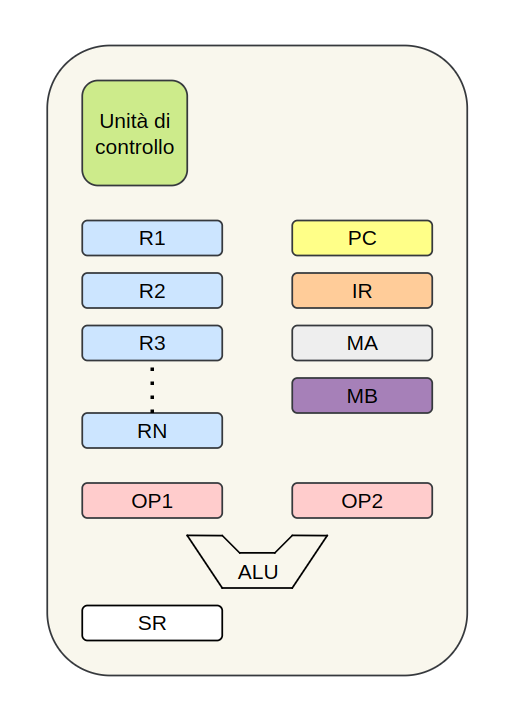
\includegraphics[width=.5\textwidth]{img/processore.png}
    \caption{Architettura di un processore generico}\label{img:processore}
\end{figure}

Oltre che la sua architettura interna, il processore è caratterizzato anche dal flusso di esecuzione di una specifica istruzione. Tale flusso può cambiare di architettura in architettura e sarà oggetto di approfondimento per i prossimi paragrafi

\newpage
\section{Architettura dei Processori moderni}
La classica architettura di un processore, riguardo l'esecuzione delle istruzioni, è poco efficiente, poichè bisogna aspettare sempre il termine di un istruzione per eseguire quella successiva.
Per velocizzare tale tipologia di sistema abbiamo 2 principali strade:
\begin{itemize}
    \item \textbf{Elettronicamente}: Si aumenta la frequenza di clock all'interno del nostro sistema (in gergo si utilizza il termine Overclock). Tale soluzione, per quanto semplice, è molto pericolosa, poichè dopo una certa soglia, non posso più aumentare la frequenza di clock. Aumentare troppo il clock potrebbe far danneggiare i componenti per la troppa energia da dissipare e quindi bisognerebbe prevedere anche delle architetture costruite ad-hoc;
    
    \item \textbf{Architetturalmente}: Vado a modificare l'architettura per gestire un nuovo modo di funzionamento del classico flusso di funzionamento di un processore. Tale modifica permetterebbe di poter eseguire più istruzioni contemporaneamente. Le tipologie di approcci che si possono avere in base a questa soluzione sono 2:
    \begin{itemize}
        \item \textbf{Parallelismo livello di Processo}: Ho a disposizione più processori (parallelismo esplicito) che vanno ad eseguire in maniera concorrente tali processi;
        \item \textbf{Parallalismo livello istruzione}: Un singolo processore riesce ad eseguire più istruzioni in maniera parallela;
    \end{itemize}
\end{itemize}

Le due macrosoluzioni non sono mutuamente esclusive, quindi si potrebbe anche pensare di effettuare una combinazione di esse.
Guardando nello specifico alla soluzione di tipo \textbf{Architetturale} si possono incontrare varie strade per poter implementare il parallelismo delle istruzioni.
Per poter meglio comprendere come effettuare la suddivisione del lavoro tramite le varie architetture, bisogna comprendere bene come strutturare un \textbf{Processo}. Tale entità la possiamo vedere come:
\begin{itemize}
    \item Formata da più task disgiunti ed indipendenti;
    \item Formata da un solo programma che richiede un'esecuzione ad elevate prestazioni.
\end{itemize}

Le architetture che negli anni sono state progettate per la distribuzione del carico di lavoro, dato da un singolo processo sono varie (quindi ci troviamo nel secondo caso).
Le tipologie principali sono:
\begin{itemize}
    \item \textbf{SISD (Single Istruction Single Data)}: Architettura in grado di eseguire una istruzione alla volta lavorando su dati singoli. Tale tipologia di architettura rispetta per filo e per segno la classica architettura di Von Neumann, la tipologia di parallelismo che si può implementare su tali sistemi è solo tramite un cambio di contesto, quindi definendo uno scheduling.
    \item \textbf{SIMD (Single Istruction Multiple Data)}: Architettura progettata per l'esecuzione di una singola istruzione su più dati. Tale tipologia di architettura è molto buona per l'esecuzione di prodotti vettoriali. Il parallelismo di tale macchina è intrinseco rispetto ai dati, poichè si agisce effettuando una singola istruzione sui vari dati.
    \item \textbf{MISD (Multiple Istruction Single Data)}: (Tali architetture sono state aggiunte solo per conoscenza personale, ma non sono state spiegate dal professore) Architettura in grado di eseguire una moltitudine di istruzioni su di un singolo dato. Tale tipologia di architettura è la meno utilizzata, poichè si cerca di eseguire sempre delle operazioni contemporanee rispetto ai dati.
    \item \textbf{MIMD (Multiple Istruction Multiple Data)}: Architettura che consente di eseguire più istruzioni su più dati. Essi eseguono quindi in parallelo, più istruzioni diverse su più dati diversi. Esse sono le più complicate per via della condivisione della memoria, difatti, ve ne sono varie, in base a come si vadano ad accedere i vari dati in memoria.
\end{itemize}

Nel nostro caso, il Motorola 68k è una tipologia di sistema \textbf{SISD}.
Ad oggi i sistemi maggiormente utilizzati sono i sistemi \textbf{MIMD}, che prevedono l'utilizzo di più unità di elaborazione per poter determinare uno specifico risultato. Tali sistemi, come detto in precedenza, possono essere di vario tipo e possono essere strutturati in vario modo.
Un primo approccio è quello di costruire due sistemi "gemelli", ovvero, costruire due calcolatori differenti che tramite la comunicazione I/O gestiscono le varie operazioni da effettuare. Tale sistema, però, non è molto efficente, poichè le comunicazioni tramite dispositivi di I/O non è veloce come i processori, per cui si avrebbe un rallentamento delle operazioni.
Per sopperire a tale problema, allora si potrebbe pensare di utilizzare un sistema di memoria condivisa tra i due processori, in modo da evitare i dispositivi di I/O. La problematica che si andrebbe a presentare in quest'altro caso sarebbe l'accesso al BUS, che nonostante sia velocissimo, ha bisogno di una buona comunicazione tra i due processori.
Per migliorare ancora tale tipologia di architettura, allora, si potrebbe pensare di utilizzare una gerarchia di memorie, che permetta di ridurre gli accessi in memoria pilotati dai vari processori, che possono lavorare sulle loro memoria "private" in maniera del tutto autonoma e concorrente senza dover schedulare l'accesso al BUS.

\begin{figure}
    \centering
    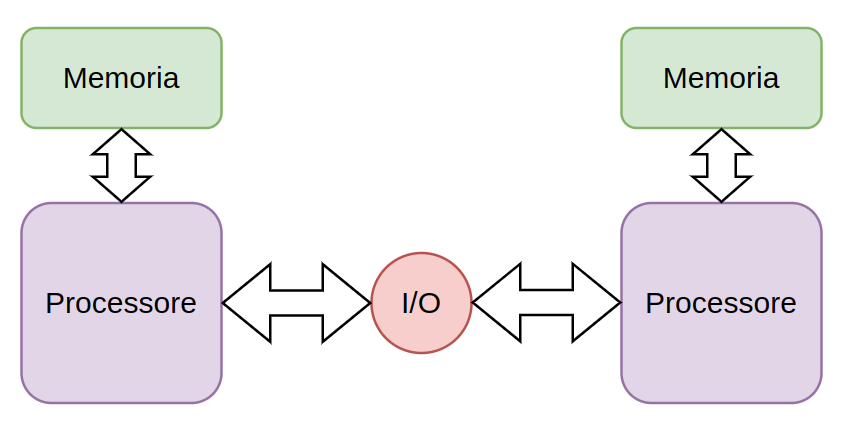
\includegraphics[width=.5\textwidth]{img/P-IO-P.png}
    \caption{Sistemi "gemelli" o sistema multicomputer}\label{img:multi-computer}
\end{figure}

\begin{figure}
    \centering
    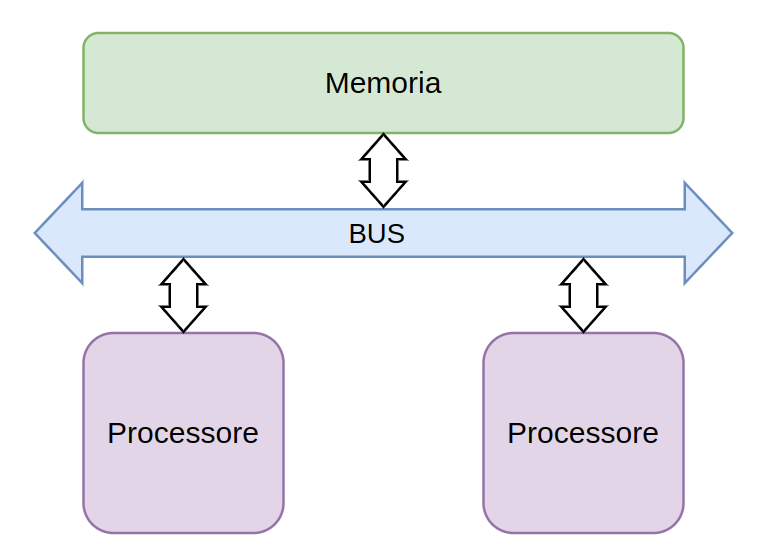
\includegraphics[width=.5\textwidth]{img/P-BUS-P.png}
    \caption{Sistema a memoria condivisa}\label{img:shared-memory}
\end{figure}

\begin{figure}
    \centering
    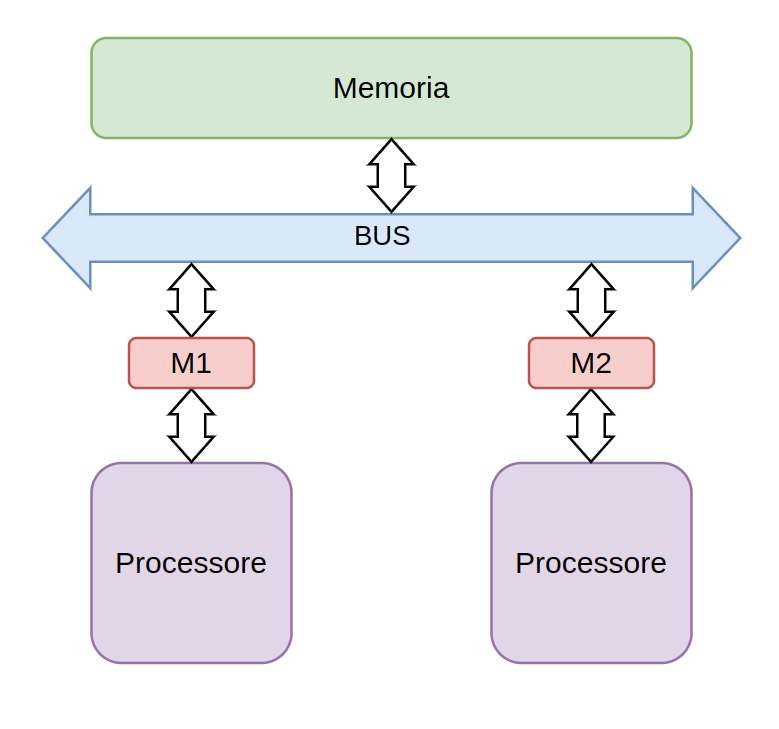
\includegraphics[width=.5\textwidth]{img/P-M-BUS-M-P.png}
    \caption{Sistema multicore}\label{img:multi-core}
\end{figure}

I sistemi che sfruttano le gerarchie di memoria prendono il nome di \textbf{sistemi multicore}, che non hanno solo 2 livelli di gerarchia di memoria, ma ne hanno vari, in base ai casi.

\newpage
\subsection{Multi-Computer e Multi-Processore}
Concentriamo la nostra attenzione sui sistemi MIMD. Escludendo la possibilità di avere un parallelismo interno, è possibile individuare due categorie di sistemi che permettono a più processori di lavorare su dati diversi, questi sono detti Multi-Computer e Multi-Processore.
\\
Un primo metodo utile a far interagire due (o più) sistemi differenti è introdurre un intermediario, ovvero un particolare tipo di sistema di I/O che sia efficace e veloce. In tal caso, quanto più rapidi saranno i processori, tanto più dovrà esserlo il sistema (oltre che la rete che li interconnette). La limitazione principale di tale modello è la sensibilità ai limiti tecnologici dovuti all'interconnessione. Il sistema globale è detto \textbf{Multi-Computer} ed è particolarmente utilizzato per applicazioni che richiedono calcoli dedicati [\ref{fig:multi-computer}].
\begin{figure}[!ht]
    \centering
    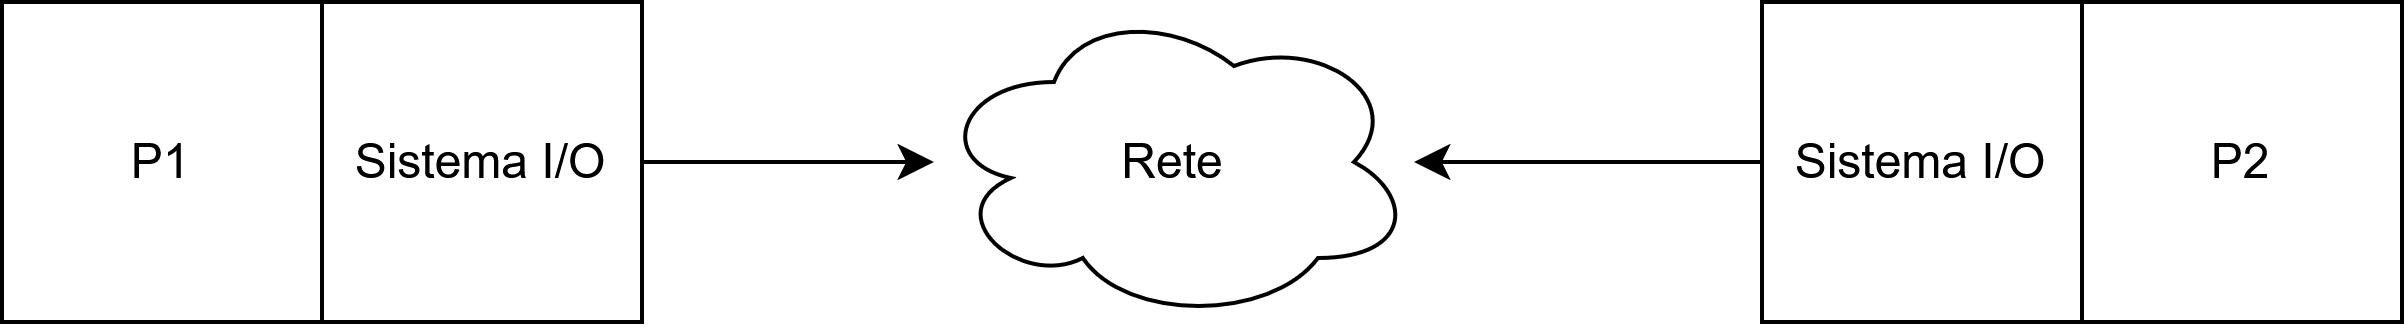
\includegraphics[width=0.8\linewidth]{img/multi-processore.png}
    \caption{Architettura di un sistema Multi-Computer.}
    \label{fig:multi-computer}
\end{figure}

Un'altra possibilità per far interagire i processori è direttamente tramite la memoria, ottenendo un sistema complessivo detto \textbf{Multi-Processore} [\ref{fig:multi-processore}]. In tal caso, la comunicazione tra i processori avviene direttamente tramite bus, superando il problema legato alla fisica realizzabilità di connessioni su larga scala. Il vantaggio di questi sistemi è che i dati possono essere trasferiti molto rapidamente in memoria grazie al bus, mentre lo svantaggio è relativo alla competizione tra i processori negli accessi in memoria. Una possibile miglioria all'architettura proposta consiste nell'integrare a ciascun processore una memoria interna più piccola che gli permetta di gestire le istruzioni. In altre parole, è necessario gestire una gerarchia delle memoria. 
Potremmo (erroneamente) pensare che aggiungere più core permetta di velocizzare il sistema, in realtà questo è sbagliato perché complicherebbe notevolmente le connessioni del bus, il quale diventerebbe il collo di bottiglia del modello.
\begin{figure}[!ht]
    \centering
    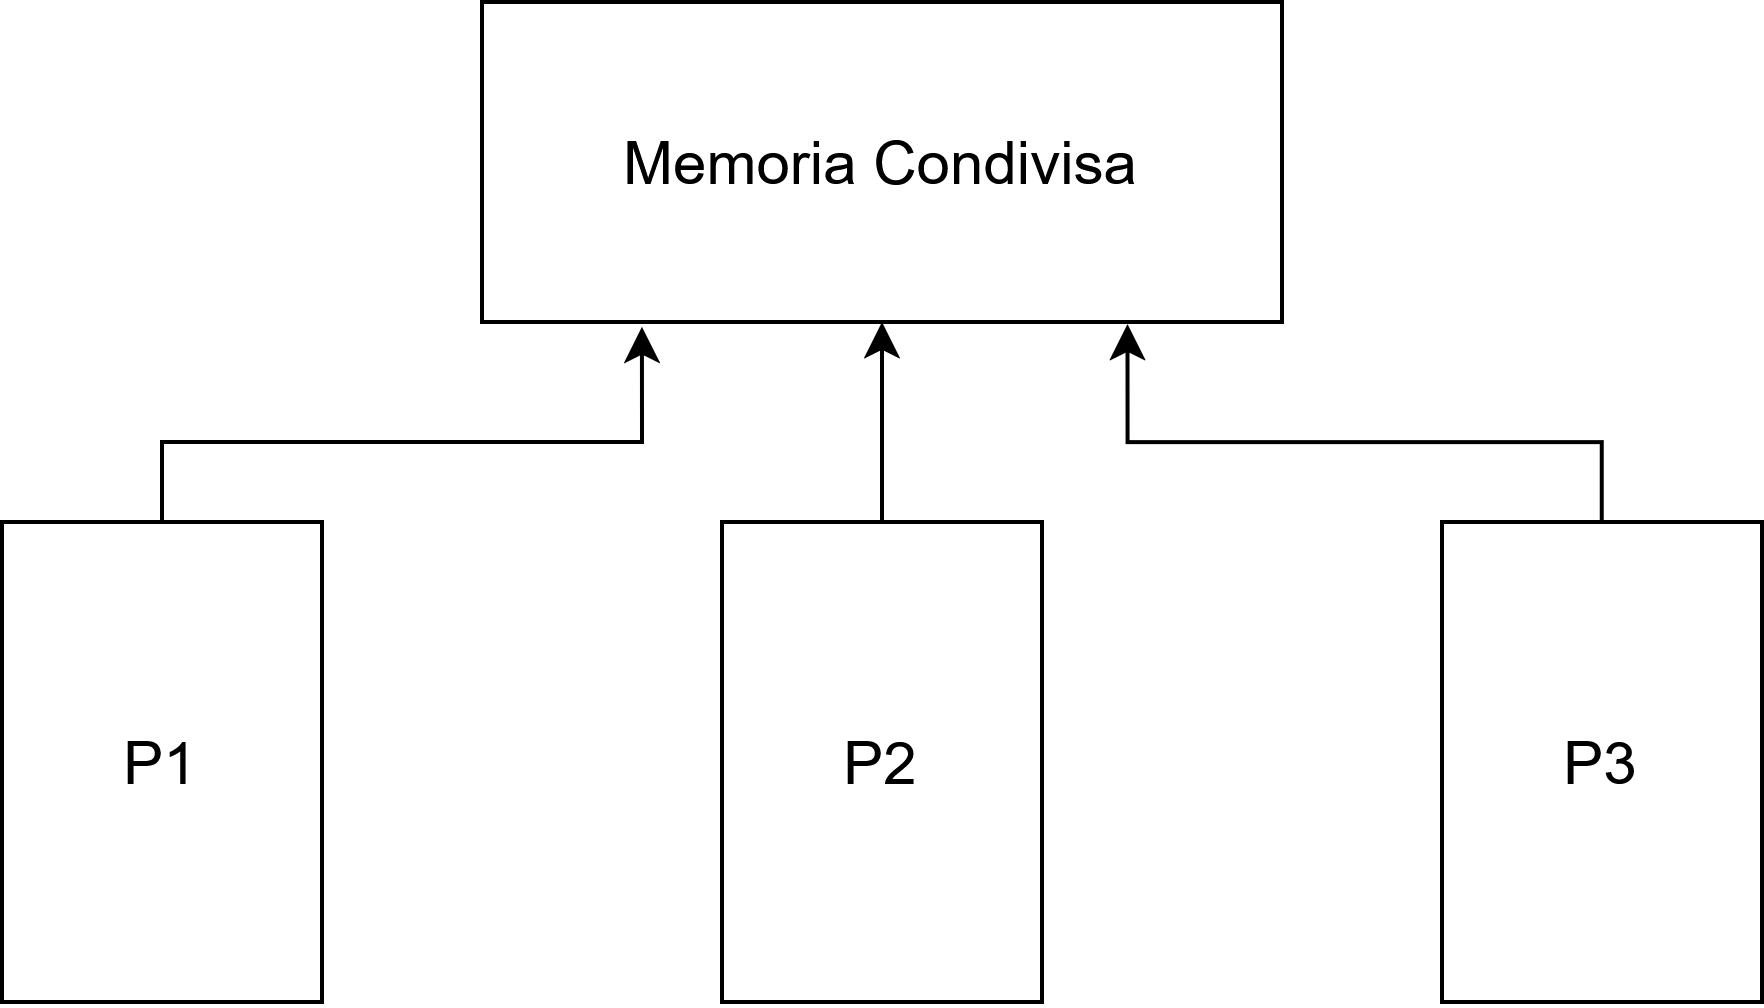
\includegraphics[width=0.5\linewidth]{img/multi-computer.png}
    \caption{Architettura di un sistema Multi-Processore.}
    \label{fig:multi-processore}
\end{figure}
L'esistenza di un modello non esclude la possibilità di inserirne un altro, cosa che accade tipicamente nei sistemi moderni.



\section{Topologia di interconnessione}
Poniamoci ora nel caso di architetture multicomputer, in cui a differenza di quelle multiprocessore, non esiste memoria condivisa né un bus comune, ma la comunicazione tra i processori dipende dalla \textbf{topologia di rete}, in particolare dal diametro (massima distanza tra due nodi).
Questo rende più complesso ridurre i costi di comunicazione, poiché spesso non è possibile ottenere una totale connettività. Un'ulteriore difficoltà riguarda l'allocazione dei processi: quando i processi sono più dei processori, è necessario bilanciare la comunicazione e l’uso delle risorse.
Idealmente, si dovrebbero:
\begin{itemize}
    \item Assegnare allo stesso nodo i processi che comunicano spesso.
    \item Distribuire su nodi diversi quelli che richiedono molte risorse computazionali.
\end{itemize}
Per ottimizzare l'allocazione servono funzioni obiettivo specifiche, ma la loro definizione è complessa perché dipende dai dati trattati dai processi.
\\
\\
Nell'ottica in cui ci poniamo (punto di vista puramente hardware), la configurazione descritta 
dall'architettura non può risolvere il problema dall'allocazione dei processi, ma può far fronte a 
quello della connettività, cercando di rendere quanto più semplice possibile la comparazione tra 
grafo del problema e quello dell'architettura.  
Esistono due soluzioni, le \textit{reti dirette} e \textit{reti indirette}.
\\
\\
Le \textbf{reti dirette} definiscono una topologia fissa, per cui la compatibilità tra i grafi è realizzata in maniera analitica attraverso l'utilizzo di formule provenienti dal campo della ricerca operativa. Le \textbf{reti indirette}, invece, sono realizzate attraverso particolari dispositivi chiamati 
\textit{switch}, che consentono di ottenere una totale connettività attraverso un 
sistema dinamico di comunicazione. Per capire meglio come questo sia possibile, è necessario approfondire alcuni dettagli di realizzazione sugli switch. Innanzitutto, l'obbiettivo principale di questi dispositivi è gestire dei conflitti, ovvero di situazioni in cui due o più nodi cercano di comunicare contemporaneamente con un altro. A questo proposito, è possibile classificare gli switch in due categorie:
\begin{itemize}
    \item A \textbf{singolo stadio} (Diretti).
    \item A \textbf{N stadi} (Indiretti).
\end{itemize}
Per creare uno \textbf{switch a connessione diretta} tra due nodi diversi, è necessario avere due informazioni: l'indirizzo del nodo sorgente e quello del nodo destinazione. Il dispositivo che si vuole realizzare dovrà avere \(N\) nodi in ingresso ed \(N\) nodi in uscita. Per poter implementare tale architettura si deve scomporre il sistema in due sottosistemi diversi, quello di ingresso e quello di uscita. Tale suddivisione viene realizzata mediante multiplexer e demulitplexer, entrambi generalmente realizzati in logica three-state [\ref{fig:switch-dir}]. 
\begin{figure}[!h]
    \centering
    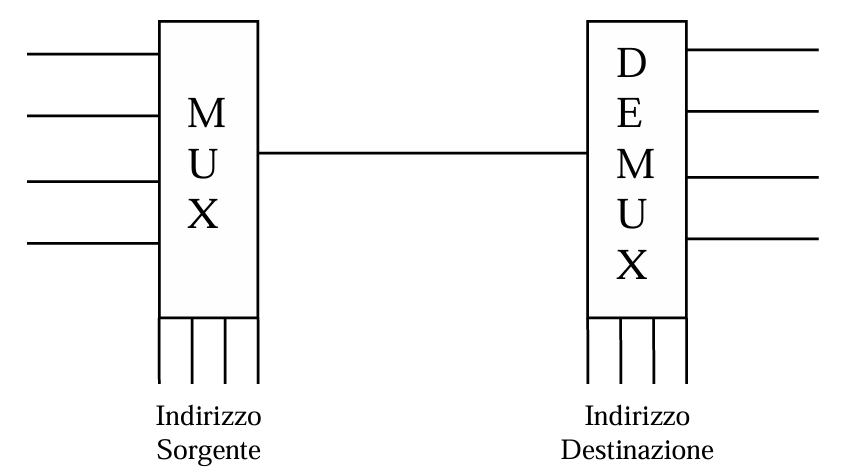
\includegraphics[width=0.35\linewidth]{img/switch_dir.png}
    \caption{Switch a singolo stadio.}
    \label{fig:switch-dir}
\end{figure}
L'inconveniente implicito del meccanismo implementato, è che automaticamente si realizza una mutua esclusione tra i nodi dovuta al fatto che, potrà essere attivo un solo collegamento per volta. Quindi, per realizzare un collegamento di \(N/2\) comunicazioni simultanee, si dovrà replicare l'hardware \(N/2\) volte. Le caratteristiche che rendono favorevole questa soluzione sono: assenza di stadi intermedi, buona efficienza, basso parallelismo e parallelismo fisico ottenuto riproducendo lo stesso elemento più volte.
\\
\\
La soluzione trovata non è esente dal problema dei conflitti, poiché aumentando il parallelismo in 
hardware si va semplicemente a rendere possibile la comunicazione parallela, ma se i nodi di 
ingresso vogliono comunicare con lo stesso nodo di uscita è inevitabile che si creano collisioni. 
Si rende necessario, quindi, predisporre un gestore dei conflitti. La soluzione con \textbf{switch indiretti}, si basa su una serie di stadi intermedi per stabilire la comunicazione tra più nodi. Sono state proposte nel tempo varie topologie per implementare tale logica, ad esempio è facile rendersi conto che, utilizzando dispositivi a due ingressi e due uscite per realizzare gli stadi, con 
\(Log_2n\) stadi è possibile risolvere il problema della connettività, avendo tra l'altro il vantaggio di usare blocchi molto semplici che devono solo decidere se 
procedere in una direzione o in un'altra. Ovviamente esiste un problema non banale, come si fa a collegare i blocchi tra di loro (indirizzamento)?. Per switch a connessione diretta l’indirizzamento è semplice perché gli indirizzi vanno direttamente nel multiplexer e nel demultiplexer per creare il path. Nel caso di architetture multistadio invece, l'indirizzo disposto in \(k\) bit, deve essere diviso in tante parti quanti sono gli stadi, in modo da comandare opportunamente i blocchi. Questo significa che non esiste una logica di controllo centralizzata come nel caso precedente, ma la logica di controllo è distribuita negli stadi. Ovviamente è una condizione abbastanza forte dal punto di vista dell'architettura, che è possibile realizzare soltanto utilizzando particolari proprietà topologiche della rete. Un esempio che implementa una soluzione molto interessante è rappresentata dalla \textbf{Omega Newtork}, la quale si basa sul concetto del \textit{perfect shuffling} [\ref{fig:omega}].  
\begin{figure}[!h]
    \centering
    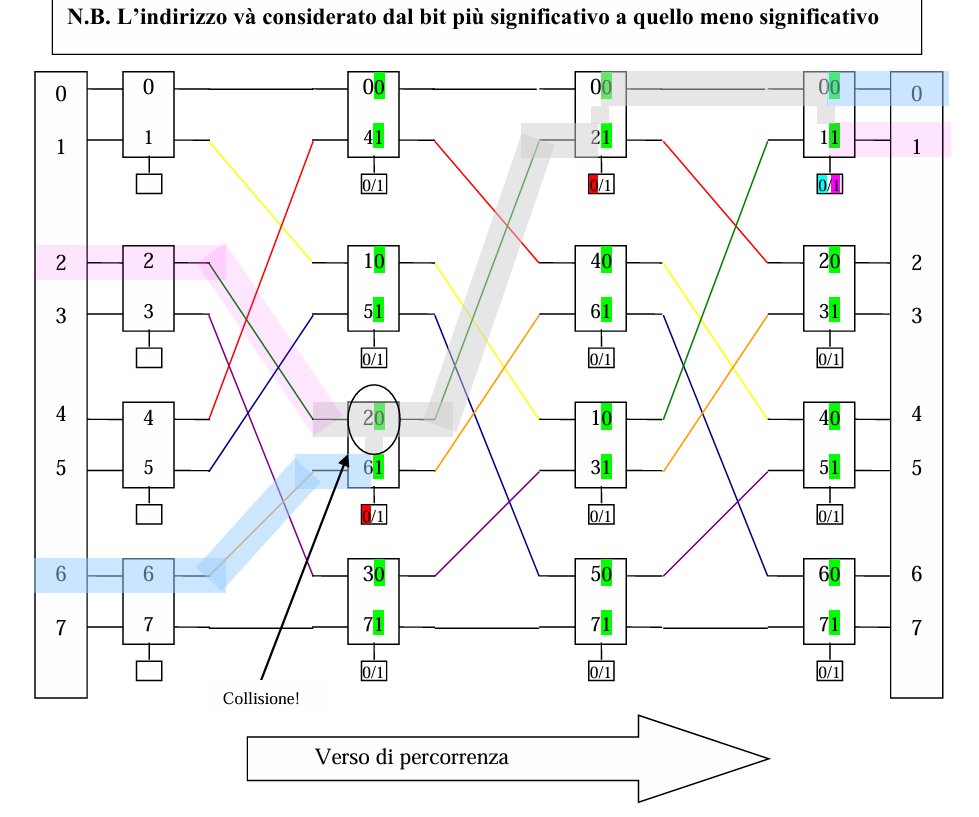
\includegraphics[width=0.6\linewidth]{img/omeganet.png}
    \caption{Switch a \(N\) stadi con omega network.}
    \label{fig:omega}
\end{figure}
Il vantaggio evidente, come detto prima, risiede nella semplicità dei componenti usati per realizzare il dispositivo che implementa il routing, ovvero blocchi con due ingressi e due uscite. L’unica nota negativa, invece, risulta proprio l'utilizzo di più stadi. Va notato che, la flessibilità indotta dall'architettura, grazie alla forte modularità dei componenti, rende lo switch molto scalabile, infatti  è facile realizzarne uno di grandi dimensioni, cosa che non è semplicemente possibile per gli switch diretti. Il problema che si verifica è, però sempre lo stesso, se due nodi di ingresso vogliono parlare con lo stesso nodo di uscita simultaneamente generano un conflitto, inoltre la contesa può anche avvenire nei nodi intermedi. Per comprendere come gestire tali conflitti, ricordiamo che la comunicazione può avvenire secondo due modalità:
\begin{itemize}
    \item \textbf{Wormhole}: Il pacchetto viene suddiviso in piccole unità, appena la prima (di solito l’header) arriva a uno switch, può essere subito inoltrata anche se il resto del pacchetto non è ancora arrivato. Lo svantaggio è che può provocare deadlock se molti pacchetti competono per le stesse risorse. I vantaggi sono una latenza più bassa (opo che l'header ha conquistato il canale i successivi frammenti viaggiano senza ritardi) e buffer di dimensioni minori. Cosa accade se il flusso di frammenti si blocca, ad esempio a causa di un conflitto? Esistono quattro soluzioni:
    \begin{enumerate}
        \item \textbf{Blocco conservativo}: Il messaggio si ferma finché il problema non si risolve. È semplice ma può bloccare molti nodi. 
        \item \textbf{Distruzione del messaggio}: Il messaggio viene eliminato. Rete con possibile perdita di dati.
        \item \textbf{Re-instradamento}: Si cerca un percorso alternativo, ma è possibile solo in reti non statiche e con topologie flessibili (quindi non per omega network). Inoltre, in questo caso i pacchetti possono arrivare fuori ordine, quindi serve una strategia software che si occupi di riordinarli. 
        \item \textbf{Cut-through}: Il nodo blocca memorizza temporaneamente i dati, mischiando wormhole e store and forward. Serve però un minimo di buffer (es. shift-register e contatore).
    \end{enumerate}
    \item \textbf{Store \& Forward}: Ogni nodo intermedio deve riceve interamente il pacchetto, e solo dopo lo memorizza (store) e lo inoltra (forward) al nodo successivo. Gli svantaggi sono i tempi di ritardo e la necessità di buffer per memorizzare le informazioni.
\end{itemize}
La differenza chiave tra i due è quindi che nel wormhole c'è una negoziazione del percorso, il quale è dinamico e dipende dal primo frammento, mentre nello store and forward  la negoziazione di tratta, ovvero avviene a ogni stadio.


\newpage
\section{Sistema Pipeline}
Una architettura pipeline è una tipologia di soluzione che viene implementata internamente nei processori per permettere l'esecuzione parallela di più istruzioni.
Per comprendere meglio cosa si intende per esecuzione parallela di più istruzioni, andiamo a considerare la strutturazione interna del flusso di esecuzione di una normale istruzione. L'esecuzione si divide nelle seguenti fasi (visualizzabili anche alla figura [\ref{img:pipe}]):
\begin{itemize}
    \item \textbf{Istruction Fetch (IF)}: Ovvero il prelievo dell'istruzione dalla memoria;
    \item \textbf{Decode (DEC)}: Decodifica ed interpretazione dell'istruzione;
    \item \textbf{Execute (EX)}: Esecuzione effettiva dell'istruzione;
    \item \textbf{Memory write (MW)}: Effettuo il prelievo dei dati all'interno della memoria;
    \item \textbf{Register write (RW)}: Inserisco i dati che mi interessano dai registri, in memoria. 
\end{itemize}

\begin{figure}
    \centering
    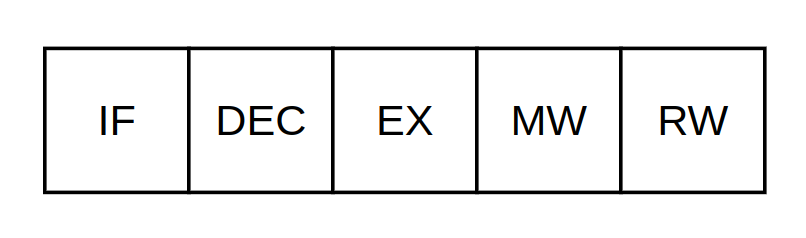
\includegraphics[width=.5\textwidth]{img/Pipeline.png}
    \caption{Architettura classica pipeline (ordine di esecuzione fasi)}\label{img:pipe}
\end{figure}

Definito il flusso di esecuzione di un' istruzione, l'architettura pipeline cerca di eseguire le fasi di un' istruzione in maniera del tutto separata, in modo da poter eseguire più fasi di istruzioni differenti. Per capire meglio questo concetto facciamo un esempio:
Devo eseguire un programma che ha 5 istruzioni, allora parto con l'esecuzione della prima fase, che preleverà l'istruzione i1, una volta prelevata, l'istruzione i1 passa alla fase di decode, mente, allo stesso istante, viene caricata l'istruzione i2 (quindi viene effettuata la Istruction Fetch dell'istruzione successiva mentre viene decodificata la precedente). Se eseguiamo tale procedura per tutte le fasi noteremo che ad ogni impulso di clock (a regime), il processore darà un risultato, quindi non ci sarà bisogno di eseguire tutte le istruzioni una per volta, poichè la suddivisione delle fasi ne permette un' esecuzione "parallela" (o meglio dire pipeline).

Per fare in modo di isolare l'esecuzione delle varie fasi, tra i vari blocchetti saranno presenti dei registri, che permettono di conservare lo stato su cui una determinata fase sta lavorando (come le architetture pipeline in elettronica [\ref{img:pipe-reg}]). 

\begin{figure}
    \centering
    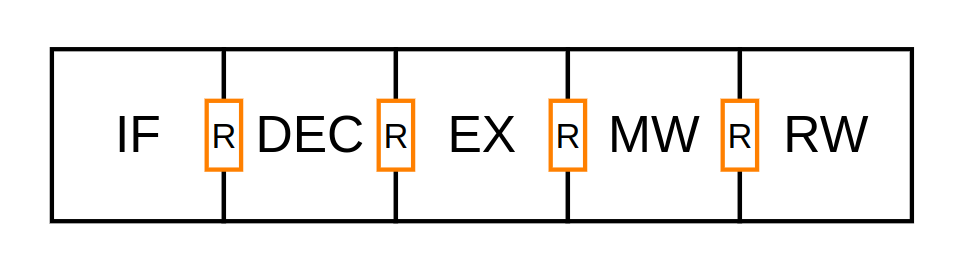
\includegraphics[width=.5\textwidth]{img/Pipe-reg.png}
    \caption{Architettura classica pipeline con registri}\label{img:pipe-reg}
\end{figure}

Un'architettura di questo tipo, però, richiede una serie di ipotesi, ovvero:
\begin{itemize}
    \item Divisione di parte dati e parte istruzioni (altrimenti dovrei gestire anche dei conflitti tra l'istruction fetch e la register/memory write);
    \item Le memorie devono avere degli accessi molto veloci: ad ogni colpo di clock viene prelevata un'istruzione e potenzialmente scritto un risultato.
    \item Le operazioni artimetico-logiche devono essere effettuate prevalentemente tra i registri interni del processore;
    \item Le istruzioni devono avere tutte lunghezza fissa;
\end{itemize}

Guardando le ipotesi possiamo capire che alcune tipologie di operazioni, che solitamente effettuevamo sul processore motorola, ora dovranno essere scompattate in varie operazioni. Un esempio classico è il comando \lstinline|ADD VAR,D1|, che utilizzava l'indirizzamento diretto per il prelievo dell'operando dalla memoria. In questo caso, però, l'indirizzamento diretto non è possibile, poichè si andrebbe ad invalidare un'ipotesi, ovvero, la lunghezza fissa dell'istruzione (che dovrebbe poi contenere l'indirizzo di memoria). Pertanto non sono previsti tutti i modi di indirizzamento.

Per comprendere meglio la problematica, consideriamo di avere un prelievo dalla memoria con un'architettura a 16-bit, ma con il memory address ed il memory buffer a 32-bit. Pertanto il seguente comando non sarebbe possibile: \lstinline|MOVE VAR,D0|; poichè richiederebbe il prelievo dell'indirizzo di memoria da 32-bit dalla memoria, ma per effettuare tale operazione, avendo solo 16 bit, avrei bisogno di due istruzioni che caricano, una i primi 16-bit e l'altra i restanti 16. Tale suddivisione, però non viene fatta dal programmatore, ma dal compilatore. Ci sono varie istruzioni che sono come la MOVE, tali istruzioni sono dette pseudo-istruzioni, poichè il compilatore andrà a suddividerle in più operazioni differenti al fine di raggiungere il risultato desiderato.

Questa cosa ci permette di capire, a questo punto, la suddivisione tra architettura di tipo CISC e architetture di tipo RISC. Le architetture di tipo CISC permettono l'esecuzione di istruzioni che sono più articolate, ma a costo di una complessità architetturale maggiore, mentre nelle architetture RISC, data la semplicità dell'architettura, le tipologie di operazioni che si possono effettuare sono ridotte ma più veloci.

\subsection{Modelli di sistemi pipeline}
Il sistema pipeline, dato il suo sistema di funzionamento, può introdurre varie tipologie di problematiche. Negli anni si sono sviluppate varie tipologie di soluzioni differenti.
Le principali architetture con cui si va a contatto al giorno d'oggi sono:
\begin{itemize}
    \item \textbf{MIPS}: Tipologia di ISA sviluppata da Patterson che poi ha venduto, per cui ora la sua implemetazione è proprietaria;
    \item \textbf{RISC-V}: Tipologia di ISA molto simile al MIPS, ma open-source;
    \item \textbf{ARM}: Tipologia di ISA proprietaria, utilizzatissima in svariati amiti (particolarmente in quello industriale), la cui implementazione è proprietaria;
\end{itemize}

Nel caso particolare di questo corso, andremo a vedere il funzionamento del RISC-V facendo riferimento sempre al MIPS, per cui saranno queste le due tipologie di architetture che si andranno ad approfondire.

Le principali problematiche che bisogna affrontare all'interno di un architettura pipeline sono le seguenti:
\begin{itemize}
    \item \textbf{Interruzioni}: Quando bisogna gestire un' interruzione la gestione dell'architettura pipe si complica, poichè bisogna capire chi ha interrotto e bisogna salvare lo stato di tutte le istruzioni che stanno eseguendo, che risulta una cosa molto onerosa e complicata;
    \item \textbf{Concorrenza sui registi}: Se due istruzioni, devono utilizzare un'informazione presente nello stesso registro ad esempio: R1 = R2+R3; R0=R1+R4;  Notiamo che per eseguire la seconda istruzione vi è bisogno del completamento della prima, ma il risultato effettivo viene scritto solo alla fine del ciclo, per cui si potrebbe incorrere in vari errori;
    \item \textbf{Salti}: Quando devo effettuare un salto, se considero il caso condizionato, non so a quale ramo andrò a saltare, è quindi più complicato capire quale sarà l'istruzione successiva da eseguire;
    \item \textbf{Gestione delle pipe multiple}: ho molteplici pipe di esecuzione, che quindi richiede una loro gestione per prevenire eventuali conflitti;
\end{itemize}

Una delle problematiche che maggiormente incide è quella riguardante il salto, poichè, dato che non conosco quale sia l'istruzione successiva, vado a bloccare la pipe appena noto che ho un'istruzione di salto, ed appena è verificata la condizione, vado a prelevare tale istruzione dalla memoria. Però questa soluzione risulta molto inefficiente, poichè introduce dei periodi in cui la pipe rimane in stallo. Difatti, una soluzione che è stata trovata è quella della branch prediction, per cui vado a processare le istruzioni successive, cercando di prevedere quale sarà il branch da eseguire, solo nel caso in cui mi accorgo che sto sbagliando vado ad effettuare il blocco della pipe, altrimenti continuo con la normale esecuzione del programma.

\subsection{Architettura del MIPS}
Il MIPS (Microprocessor without Interlocked Pipelined Stages) è una tipologia di architettura Pipelined di tipo RISC.
Nel precedente capitolo abbiamo visto le fasi di esecuzione di un'architettura pipelined generale [\ref{img:pipe}], però, nel caso del MIPS, tali fasi variano leggermente. Difatti il MIPS è caratterizzato dalle seguenti fasi:
\begin{itemize}
    \item \textbf{Istruction Fetch}: Prelievo dell'istruzione dalla memoria e incremento del program counter;
    \item \textbf{Decode}: Si vanno a prelevare gli operandi dall'istruction file e si preparano i segnali di controllo per la fase di esecuzione;
    \item \textbf{Execute}: Esecuzione delle operazioni logico-aritmetiche pilotate dai segnali della fase di decode precedente;
    \item \textbf{Memory}: Vado a leggere o scrivere qualcosa dalla memoria e gestione dei Salti;
    \item \textbf{Write Back}: Accedo in scrittura al register file per scrivere i risultati ottenuti;
\end{itemize}

Come per tutte le architettura pipelined, anche il MIPS richiede che tra le varie fasi vi siano dei registri che conservino lo stato dell'operazione.
Il MIPS, pertanto, presenta vari casi di conflitto che richiedono delle ipotesi sul sistema stesso. Tali ipotesi sono:
\begin{itemize}
    \item \textbf{Velocità della memoria}: La memoria che sarà utilizzata dal MIPS sarà acceduta molto frequentemente (precisamente 5 volte in più rispetto al caso senza pipe);
    \item \textbf{Concorrenze sulla memoria}: Presenza di due memorie, una per le istruzioni ed una per i dati. Tali memorie vengono previste per evitare la concorrenza tra la fase di fetch (prelievo dell'istruzione dalla memoria) e la fase di MEM (lettura o scrittura dalla memoria);
    \item \textbf{Concorrenza sui registri}: Si prevede che la fase di Decode sia eseguita nella seconda parte del ciclo clock, mentre la fase di write back nella prima parte del ciclo di clock. Tale presupposizione viene fatta, per evitare la concorrenza sui registri che interessano l'operazione, e quindi evitare conflitti indesiderati.
\end{itemize}

\subsubsection{Fase di Fetch}
La fase di fetch è caratterizzata da 2 principali operazioni, la fase di prelievo dell'indirizzo e la fase di incremento del program counter. Pertanto la sua parte architetturale è formata dalle componenti:
\begin{itemize}
    \item \textbf{ADD}: Strumento aritmetico per l'incremento del program counter (differente dal componente di ALU);
    \item \textbf{MUX}: Seleziona se considerare l'indirizzo di memoria successivo del program counter o un registro di memoria dettato dalla fase di MEM;
    \item \textbf{PC}: Registro program counter;
    \item \textbf{Istruction Memory}: Vado a prelevare l'istruzione da eseguire dalla memoria;
\end{itemize}

\subsection{Fase di Decode}
Nella fase di Decode, il MIPS, va a decodificare ed interpretare il comando. Le parti che compongono l'architettura della fase di decode sono:
\begin{itemize}
    \item \textbf{Registers}: Registri interni del processore che possono essere pilotati sia in lettura che in scrittura tramite dei segnali esterni (contenuti nella sotto-architettura);
    \item \textbf{Sign-extend}: Blocco di estensione con segno dei possibili valori immediati contenuti nell'istruzione;
\end{itemize}

\subsection{Fase di Execute}
Nella fase Execute viene eseguita effettivamente l'istruzione. La parte architetturale è composta da vari componenti interessanti
\begin{itemize}
    \item \textbf{Add}: Strumento che viene utilizzato per calcolare un eventuale offset rispetto ad un valore;
    \item \textbf{Shift left 2}: Vado a moltiplicare per 4 il valore per cui voglio saltare (in modo da saltare a 4 indirizzi più avanti);
    \item \textbf{ALU}: Strumento di calcolo aritmetico;
    \item \textbf{Multiplexer}: Vedo se devo selezionare il dato immediato o un secondo dato proveniente da un registro;
\end{itemize}

\subsection{Fase di Mem}
Nella fase di memorizzazione vado ad interagire con la memoria per effettuare o operazioni di lettura o operazioni di scrittura
La sua architettura è composta principalmente dal singolo elemento di accesso alla memoria dati

\subsection{Fase di Write Back}
In tale fase vado a verificare cosa bisogna scrivere all'interno dei registri interni. Il componente che meglio indica il suo funzionamento è il multiplexer finale che serve per specificare se il dato da caricare all'interno dei registri sia il risultato dell'ALU o qualche valore proveniente dalla memoria

\subsection{Registri Intermedi}
I registri che sono posti tra una fase e l'altra della pipeline sono molto più complessi di quel che si crede. Essi non contengono solo dati informativi (operandi e risultati), ma contengono anche: traccia dell'operazione da effetture, destinazione del risultato ecc. 
L'architettura e le componenti di cui si è parlato sopra, quindi, sono solo una parte di quello che è effettivamente stato realizzato sull'hardware del dispositivo.
La schematizzazione che abbiamo fatto ci permette di capire bene il funzionamento di un sistema pipeline senza entrare troppo nei dettagli della sua implementazione hardware

\subsection{Gestione dei Salti}
L'architettura pipeline ha una criticità di cui abbiamo già attentamente discusso in precedenza, i salti.
Quando sopraggiunge un istruzione di salto, riusciamo a captare che è così solo nella fase di esecuzione dell'istruzione, e quindi, se dovessimo aggiustare il PC seguendo tutta la pipe, dovremmo aspettare la fase di write back. Ma per evitare tale situazione, andiamo a retroazionare la fase di esecuzione con la fase di Istruction Fetch. Tale retroazione permette di capire quando e dove poi si andrà a saltare. Ciò però deve prevedere il sacrificio o l'introduzione di un istruzione "vittima", tale istruzione sarà eseguita indipendentemente a dove si andrà a saltare. Tale istruzione è la no-operation (NOP), che viene inserita subito dopo la JMP per evitare la perdita di eventuali istruzioni utili.
Tale soluzione è molto buona quando lavoro con il MIPS, poichè questo è caratterizzato dalla sua particolare pipe molto corta (e quindi molto RISC), ma nei processori più moderni, posso avere delle pipe molto più profonde ed articolate. Una soluzione alternativa a quella proposta precedentemente è quella di utilizzare la branch-prediction

\subsubsection{Branch prediction}
La branch prediction è una tecnica che cerca di prevedere a quale ramo un istruzione di salto condizionato possa saltare. Tale tecnica valuta le prestazioni in base a quanto si possa "perdere" in termini di efficienza (ricaricare il branch corretto rispetto a quello predetto).
Per capire bene questa cosa andiamo a considerare il seguente pseudocodice:
\begin{lstlisting}[language=C]
for (int i = 0; i < N; i++){
    for (int j = 0; j < N; j++){
        operazioni
    }
}
\end{lstlisting}

Tali for prevedono un controllo iniziale sulla variabile. Vedendo come sono strutturati tale controllo prevede l'esecuzione del ramo else una sola volta (guardando il for interno) ogni N passi.
I modi pre prevedere il branch possono essere vari, e possono essere descritti mediante degli appositi automi a stati finiti. Un primo approccio molto basilare è quello di andare a cambiare il branch da caricare successivamente ad ogni errore di decisione e quindi eseguire le operazioni descritte dall'automa [\ref{img:automa-semplice}].

\begin{figure}[!ht]
    \centering
    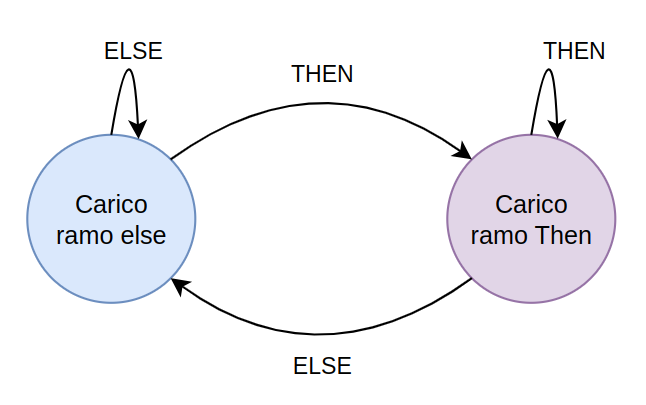
\includegraphics[width=.5\textwidth]{img/automa-semplice.png}
    \caption{Automa della branch prediction base}\label{img:automa-semplice}
\end{figure}

Tale soluzione, però, guardando al nostro caso, non è proprio ottimale, poichè per quel singolo fail che avviene ad ogni N interazioni dovrò assorbirmi 2 fault. Per evitare tale condizione, e quindi rendere la persistenza più forte, vado a costruire un automa a 4 stati che mi permette di rendere la condizione di "cambio del branch" più solida, poichè solo in caso di due fault successivi (fault = errore nel riconoscere il branch giusto), allora cambio il mio branch effettivo. L'automa che meglio spiega tale principio è quello visualizzabille all'immagine [\ref{img:automa-complesso}]

\begin{figure}[!ht]
    \centering
    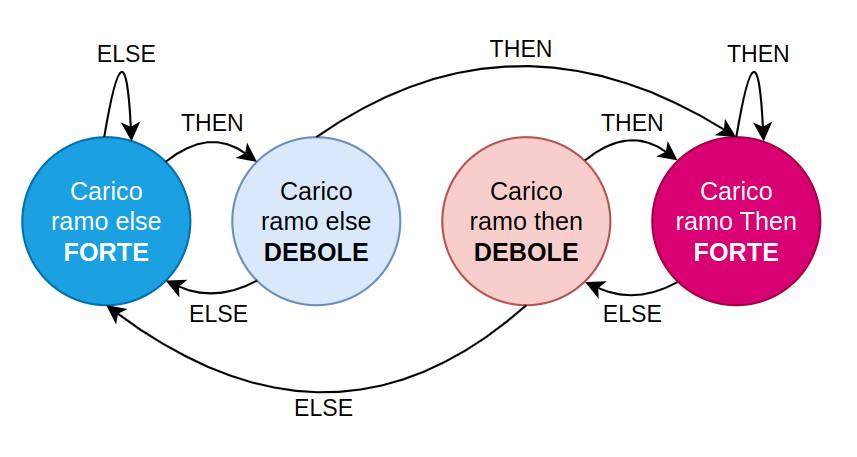
\includegraphics[width=.5\textwidth]{img/automa-complesso.png}
    \caption{Automa della branch prediction avanzato}\label{img:automa-complesso}
\end{figure}

\section{Architetture Superscalari}
L'utilizzo delle pipe porta dei vantaggi non in termini di attraversamento di una istruzione, che rimane invariato, ma in termini di produttività. Per ottenere prestazioni ancora migliori, è possibile realizzare un'architettura con più pipe che eseguono diverse istruzioni in parallelo, così da aumentare la produttività del sistema. Una tale architettura viene chiamata \textbf{Superscalare}. Tuttavia, questa introduce delle problematiche che vanno necessariamente risolte, queste sono:
\begin{enumerate}
    \item Le pipe devono condividere un unico accesso in memoria comune per il prelievo delle istruzioni. In altre parole, anche in presenza di più pipe tutte devono leggere dalla stessa memoria. Questo può creare un collo di bottiglia, perché solo una pipeline alla volta può leggere da lì.
    \item Se le pipe non sono del tutto indipendenti ma condividono delle stazioni, nascono dei problemi di conflitto nell'utilizzo delle unità funzionali condivise. Se due pipeline vogliono usare la stessa unità (ad esempio, la ALU) allo stesso momento, nasce un collisione e una delle due deve aspettare. Questo riduce l'efficienza.
\end{enumerate}

\subsection{Gestione delle Collisioni}
La \textbf{gestione delle collisioni} nella architetture superscalari avviene completamente in hardware. Per comprendere al meglio come un processore con una tale architettura gestisca il problema, introduciamo un esempio. Supponiamo che la CPU sia in grado di realizzare addizione e moltiplicazione in floating point. Come possiamo immaginare, alcune delle operazioni presenti nell'addizione potrebbero essere richieste anche dalla moltiplicazione (e viceversa), mappiamo dunque all'interno di una tabella le diverse operazioni necessarie a completare le due [\ref{tab:mul} e \ref{tab:add}].

\begin{table}[!h]
\centering
\begin{tabular}{|l|c|c|c|c|c|c|c|}
\hline
         & 1 & 2 & 3 & 4 & 5 & 6 & 7 \\
\hline
Ex Add   & X &   &   &   &   &   &   \\
\hline
Mult     &   & X & X &   &   &   &   \\
\hline
Man Add  &   &   & X & X &   &   &   \\
\hline
Renorm   &   &   &   &   & X &   & X \\
\hline
Round    &   &   &   &   &   & X &   \\
\hline
Shift A  &   &   &   &   &   &   &   \\
\hline
Lead 1   &   &   &   &   &   &   &   \\
\hline
Shift B  &   &   &   &   &   &   &   \\
\hline
\end{tabular}
\caption{7 stadi richiesti dalla moltiplicazione.}
\label{tab:mul}
\end{table}

\begin{table}[!h]
\centering
\begin{tabular}{|l|c|c|c|c|c|c|c|c|c|}
\hline
         & 1 & 2 & 3 & 4 & 5 & 6 & 7 & 8 & 9 \\
\hline
Ex Add   & X &   &   &   &   &   &   &   &   \\
\hline
Mult     &   &   &   &   &   &   &   &   &   \\
\hline
Man Add  &   &   &   & X &   &   &   &   &   \\
\hline
Renorm   &   &   &   &   &   &   &   &   & X \\
\hline
Round    &   &   &   &   &   &   &   & X &   \\
\hline
Shift A  &   & X & X &   &   &   &   &   &   \\
\hline
Lead 1   &   &   &   &   & X &   &   &   &   \\
\hline
Shift B  &   &   &   &   &   & X & X &   &   \\
\hline
\end{tabular}
\caption{9 stadi richiesti dall'addizione.}
\label{tab:add}
\end{table}

L'introduzione di tali tabelle semplifica notevolmente la scrittura del \textbf{vettore delle collisioni}, ovvero un particolare vettore binario utilizzato dal compilatore per gestire il problema dei conflitti tra pipe. Poniamoci nell'ipotesi semplificativa di due sole pipe, in modo da visualizzare pù facilmente il processo. Per ricavare il vettore, è sufficiente sovrapporre le tabelle delle operazioni che vogliamo eseguire, opportunamente shiftate a seconda di quale delle due sia eseguita prima. Ad esempio, se vogliamo eseguire una moltiplicazione X e al ciclo di clock successivo un'altra moltiplicazione Y, la sovrapposizione delle tabelle fornisce il seguente risultato [\ref{tab:collision}].

\begin{table}[!h]
\centering
\begin{tabular}{|l|c|c|c|c|c|c|c|}
\hline
         & 1 & 2 & 3 & 4 & 5 & 6 & 7 \\
\hline
Ex Add   & X & Y &   &   &   &   &   \\
\hline
Mult     &   & X & XY & Y &   &   &   \\
\hline
Man Add  &   &   & X & XY & Y &   &   \\
\hline
Renorm   &   &   &   &   & X & Y & X \\
\hline
Round    &   &   &   &   &   & X & Y \\
\hline
Shift A  &   &   &   &   &   &   &   \\
\hline
Lead 1   &   &   &   &   &   &   &   \\
\hline
Shift B  &   &   &   &   &   &   &   \\
\hline
\end{tabular}
\caption{Collisioni tra due moltiplicazioni sfasate di 1 ciclo di clock.}
\label{tab:collision}
\end{table}
La tabella evidenzia come le due operazioni, eseguite secondo la tempificazione descritta, presentano delle collisioni al tempo 3 e 4 (presenza contemporanea di X e Y). Il corrispondente vettore delle collisioni sarà dunque 0011000. \MakeUppercase{è} fondamentale ribadire che il vettore si limita solamente a segnalare la presenza di una collisione (1 nella stringa), ma ciò non ha niente a che vedere con le fasi della pipeline. In altre parole, se nella stringa c'è un 1 nella terza posizione, questo NON significa che la collisione riguarda la terza fase.
\\
\\
\MakeUppercase{è} da notare come in tal caso non valga la proprietà commutativa, realizzando infatti prima una moltiplicazione e poi un'addizione non ci sarebbe alcune collisione. Nel nostro esempio ci siamo fermati a realizzare il collision vector per 1 solo caso, ovvero quello in cui una moltiplicazione segue una moltiplicazione. In generale, è necessario costruirlo per tutte le possibili combinazioni di operazioni (\textit{mul} segue \textit{add}, \textit{add} segue \textit{add}, eccetera). Se per ipotesi avessimo \(n\) istruzioni da realizzare, sarebbe necessario costruire \(2^n\) vettori, complicando notevolmente il lavoro del compilatore.
\\
\\
Ritorniamo all'esempio e cerchiamo di capire come il compilatore gestisca le collisioni per una generica sequenza di operazioni, che supponiamo essere: \textit{add, mul, mul}. \MakeUppercase{è} innanzitutto necessario costruire il vettore di collisione per le operazioni \textit{add-mul} e \textit{mul-mul}. A questo punto, bisogna inserire la seconda moltiplicazione tenendo conto sia della moltiplicazione precedente che della prima addizione. Tale condizione viene completamente gestita in hardware, secondo una struttura fatta nel seguente modo [\ref{fig:hardware-coll}].
\begin{figure}[!h]
    \centering
    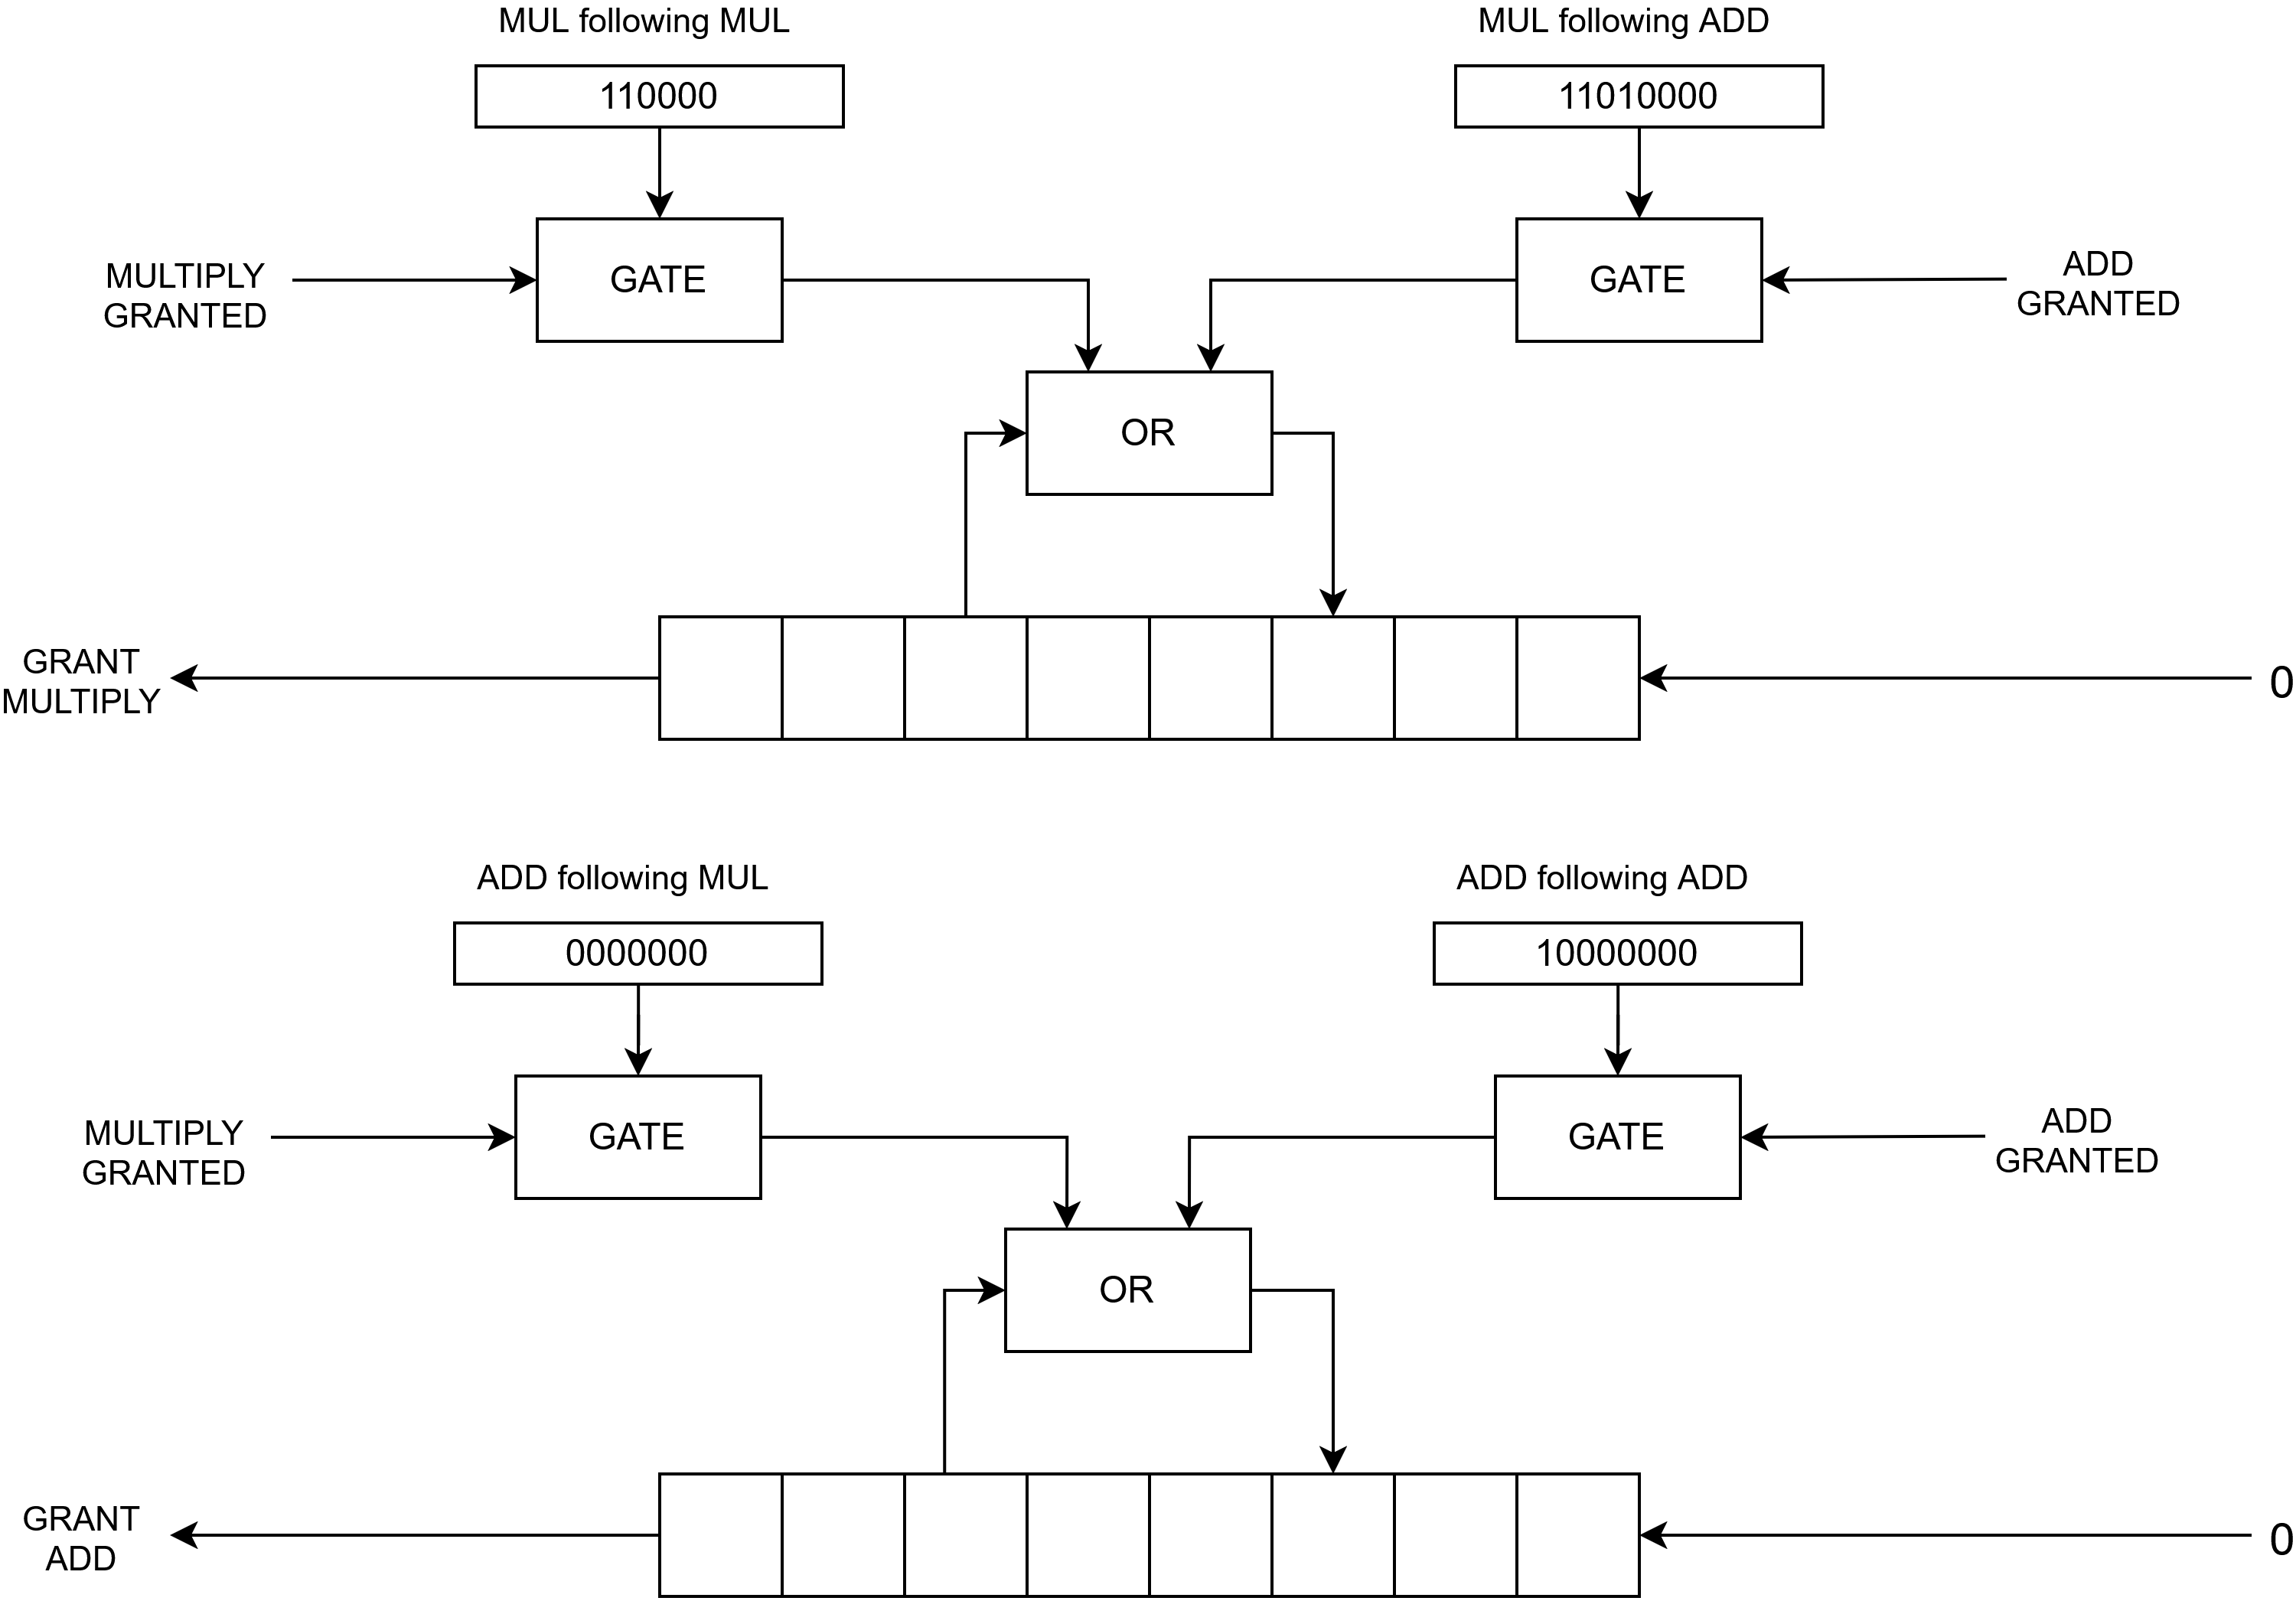
\includegraphics[width=0.7\linewidth]{img/superscalari_collisioni.png}
    \caption{Hardware per la gestione delle collisioni.}
    \label{fig:hardware-coll}
\end{figure}
In particolare, il registro a scorrimento fa proseguire la "storia" delle istruzioni, mentre la OR "unisce" la storia precedente con la nuova. Quindi, la OR garantisce che non ci sia collisione né con l'istruzione che stiamo aggiungendo, né con la storia di istruzioni precedenti. \MakeUppercase{è} fondamentale notare come la struttura sia suddivisa in due parti, quella superiore che riguarda soltanto la moltiplicazione, e quella inferiore che invece riguarda l'addizione.
\\
\\
Un tale tipo di soluzione hardware per la gestione delle collisioni è tipica dei sistemi \textbf{DSP} (Digital Signal Processor), come quelli usati per audio, video, telecomunicazioni. In particolare, il suo utilizzo permette di schedulare le istruzioni nel modo più efficiente possibile evitando stalli o rallentamenti.
